\documentclass[conference]{IEEEtran}
\IEEEoverridecommandlockouts
% The preceding line is only needed to identify funding in the first footnote. If that is unneeded, please comment it out.
\usepackage{cite}
\usepackage{amsmath,amssymb,amsfonts}
\usepackage{algorithmic}
\usepackage{graphicx}
\usepackage{subfig}
\usepackage{float}
\usepackage{textcomp}
\usepackage{xcolor}
\def\BibTeX{{\rm B\kern-.05em{\sc i\kern-.025em b}\kern-.08em
    T\kern-.1667em\lower.7ex\hbox{E}\kern-.125emX}}
\begin{document}

\title{Algoritmos de planificación de caminos\\
{\footnotesize \textsuperscript{*}}
}

\author{\IEEEauthorblockN{1\textsuperscript{st} Sergio Masa Avís}
\IEEEauthorblockA{\textit{} \\
\textit{Universidad Carlos III de Madrid}\\
Madrid, España\\
100401052@alumnos.uc3m.es}
\and
\IEEEauthorblockN{2\textsuperscript{nd} Ángel Ignacio Arnanz Paredes}
\IEEEauthorblockA{\textit{} \\
\textit{Universidad Carlos III de Madrid}\\
Toledo, España \\
100405096@alumnos.uc3m.es}
\and
\IEEEauthorblockN{3\textsuperscript{rd} Julio Sánchez Mirón}
\IEEEauthorblockA{\textit{} \\
\textit{Universidad Carlos III de Madrid}\\
Granada, España \\
100394981@alumnos.uc3m.es}
}

\maketitle

\begin{abstract}
This document is a model and instructions for \LaTeX.
This and the IEEEtran.cls file define the components of your paper [title, text, heads, etc.]. *CRITICAL: Do Not Use Symbols, Special Characters, Footnotes, 
or Math in Paper Title or Abstract.
\end{abstract}

\begin{IEEEkeywords}
component, formatting, style, styling, insert
\end{IEEEkeywords}


\section{Breadth-First Search (BFS)}

\vspace{0.2mm}

\subsection{Descripción del Algoritmo}

Se trata de una estrategia en la que se parte de un nodo ra\'iz. Este es el primero que se expande, dando lugar a nodos sucesores. Estos se expandir\'an para una profundidad dada en el \'arbol de b\'usqueda antes de que ningún nodo del siguiente nivel se expanda. De modo que el nodo menos expandido es elegido para ser el pr\'oximo en expandirse.

\begin{figure}[H]
\centerline{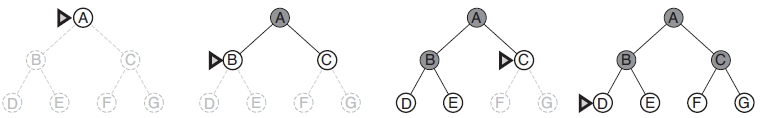
\includegraphics[scale=0.4]{IMAGENES/BFS.png}}
\caption{BFS en un \'arbol binario}
\label{fig}
\end{figure}

Esto se logra f\'acilmente debido a que se usan colas FIFO en la frontera. De manera que los nuevos nodos generados van a la parte de atr\'as de la cola mientras que los nodos antiguos, que tienen menor profundidad que los nodos nuevos, son expandidos. Este algoritmo descarta cualquier camino o conjunto ya en la frontera o conjunto explorado. Se busca siempre la ruta menos profunda para todos los nodos en la frontera ya que en cuanto el nodo es generado objetivo sabemos que todos los posibles nodos menos profundos han sido explorados.

\begin{center}
\textit{Pseudocódigo}
\end{center}

\begin{enumerate}
\item BFS (q,origen,destino,mapa)
\item \hspace{1cm} Mientras existan v\'ertices que recorrer:
\item \hspace{1cm} explored \(\rightarrow\) mapa con nodos visitados
\item \hspace{1cm} q $\rightarrow$ siguiente nodo a evaluar de la Cola
\item \hspace{1cm} Si q = destino
\item \hspace{2cm} Se ha encontrado el camino
\item \hspace{1cm} Si q != origen
\item \hspace{2cm} Generamos 4 nodos m\'as pr\'oximos
\item \hspace{1cm} Para cada hijo se comprueba que no est\'e en explored  y se encuentre dentro del mapa
\item \hspace{1cm} Metemos al hijo en la cola q
\end{enumerate}

\subsection{Propiedades}    %%%%%%%%%%%%%%%%%%% PROPIEDADES %%%%%%%%%%%%%%%%%%%%%%%


Las propiedades del algoritmo BFS son:

{\setlength{\parskip}{1em}
\begin{itemize}


\item Completo. 


Se ve f\'acilmente que es completo, si el nodo de inter\'es est\'a a una profundidad finita, d, BFS encontrará el nodo objetivo (siempre que el factor bifurcaci\'on b sea finito) tras generar todos los nodos superficiales.


{\setlength{\parskip}{1em}

\item \'Optimo. 


El nodo objetivo m\'as superficial no tiene porque ser el m\'as \'optimo, debido a que la distancia entre los nodos puede que no sea la misma. BFS es \'optimo si la ruta de coste es una función de la profundidad del nodo no decreciente. El caso m\'as com\'un es que todos los caminos tengan el mismo coste.
}


\end{itemize}
}

\subsection{Complejidad}
{\setlength{\parskip}{1em}
\begin{itemize}

\item 1)	Complejidad computacional o en tiempo. 

Suponiendo que la soluci\'on tenga una profundidad, d. En el peor caso, es el \'ultimo nodo generado en ese nivel. Siendo el número de nodos generados:

\begin{figure}[H]
\centerline{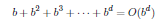
\includegraphics[scale=1]{IMAGENES/ndenodos.png}}
\caption{}
\label{fig}
\end{figure}


\item 2)	Complejidad en memoria o en espacio. 

Para este tipo de gr\'aficos de b\'usqueda, los cuales almacenan cada nodo expandido en el conjunto explorado, la complejidad en el espacio se encuentra en el factor b de la complejidad en el tiempo. Para la b\'usqueda en BFS, cada nodo generado se mantiene en memoria. En el conjunto explorado hay O(b$^{d-1}$) nodos y O(b) nodos en la frontera siendo la complejidad del espacio O(b$^{d}$). En una b\'usqueda de \'arbol no se ahorrar\'ia mucho espacio ni tiempo debido a que en el espacio de estados hay muchas rutas redundantes.

\end{itemize}
}

\section{Depth-First Search (DFS)}

\vspace{0.2mm}

{\setlength{\parskip}{1em}

\subsection{Descripci\'on del Algoritmo}

En el \'arbol de b\'usqueda siempre se expande el nodo m\'as profundo de la frontera. La búsqueda procede inmediatamente a los niveles m\'as profundos del \'arbol de b\'usqueda, los cuales no tienen sucesores. En caso de que no encuentre el nodo objetivo por esa rama realizar\'a una vuelta atr\'as al siguiente nodo con mayor profundidad que todav\'ia no haya sido explorado.

Se emplea la cola LIFO donde los nuevos nodos generados son los elegidos para su expansi\'on.

Las propiedades y complejidad del DFS depende de si se emplea la versión graph-search o tree-search. En este trabajo se ha implementado la versión tree-search.


\begin{figure}[H]
\centerline{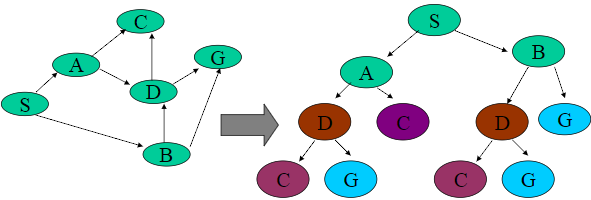
\includegraphics[scale=0.4]{IMAGENES/Graph-search_Tree-search.png}}
\caption{}
\label{fig}
\end{figure}

\begin{center}
\textit{Pseudoc\'odigo}
\end{center}

\begin{enumerate}
\item DFS (q,origen,destino,mapa)
\item \hspace{1cm} Mientras existan nodos que recorrer:
\item \hspace{1cm} explored \(\rightarrow\) mapa con nodos visitados
\item \hspace{1cm} Mientras que haya elementos en la Pila
\item \hspace{1cm} q $\rightarrow$ siguiente nodo a evaluar de la Pila
\item \hspace{1cm} Si q = destino
\item \hspace{2cm} Se ha encontrado el camino
\item \hspace{1cm} Si q != origen
\item \hspace{2cm} Generamos 4 nodos m\'as pr\'oximos
\item \hspace{1cm} Para cada hijo se comprueba que no est\'e en explored  y se encuentre dentro del mapa
\item \hspace{1cm} Metemos al hijo en la cola q
\end{enumerate}

\subsection{Propiedades}    %%%%%%%%%%%%%%%%%%% PROPIEDADES %%%%%%%%%%%%%%%%%%%%%%%


Las propiedades del algoritmo DFS son:

{\setlength{\parskip}{1em}
\begin{itemize}


\item Completo. 

No es completo, ya que la b\'usqueda del primer \'arbol en profundidad puede modificarse sin coste de memoria adicional para verificar los nuevos estados con los de la ruta desde el nodo ra\'iz hasta el nodo actual. Esto evita bucles infinitos en espacios de estados finitos, pero no evita que se creen caminos redundantes.


{\setlength{\parskip}{1em}

\item \'Optimo. 


No es \'optimo porque expande un nodo ( B ) y explora todo el sub\'arbol de este nodo ( B ) a pesar de que el nodo vecino ( C ) sea el nodo objetivo. Suponiendo que el nodo J y nodo C fuera el mismo la versi\'on DFS devolvería este camino como soluci\'on a pesar de que no fuera la mejor soluci\'on. Hasta que no eval\'ua todos los nodos generados a partir de este primero (nodo A) no ira a expandir los nodos hermanos de este primer nodo que se evalu\'o. 
}


\end{itemize}
}

\begin{figure}[H]
\centerline{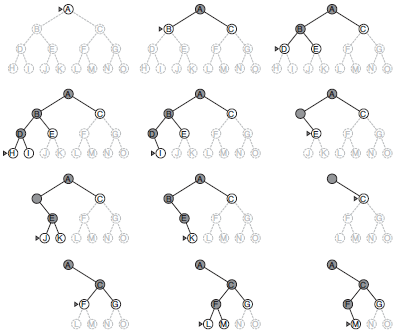
\includegraphics[scale=0.4]{IMAGENES/Tree_search_DFS.png}}
\caption{DFS en un \'arbol binario}
\label{fig}
\end{figure}

\subsection{Complejidad}
{\setlength{\parskip}{1em}
\begin{itemize}

\item 1)	Complejidad computacional o en tiempo. 

Genera todos los nodos de O($b^{m}$), donde b es el factor de ramificaci\'on y m es la profundidad m\'axima del nodo. Se ha de tener en cuenta que m puede ser mayor a d, que es la profundidad de las soluci\'on m\'as superficial.

\item 2)	Complejidad en memoria o en espacio. 

El motivo de incluir el algoritmo DFS es la complejidad en el espacio. La ventaja obtenida es que necesita almacenar \'unicamente el camino del nodo ra\'iz al nodo objetivo, junto con los nodos hermanos restantes no expandidos para cada uno de los nodos que conforman el camino. Tras ser expandido un nodo puede ser eliminado junto con sus descendientes explorados.

\end{itemize}
}



\section{Dijkstra's algorithm}

\vspace{0.2mm}

\subsection{Idea general}

Al igual que en los métodos descritos previamente, estamos ante un algoritmo (`no-informado') clásico de búsqueda de caminos entre dos nodos de un grafo. La peculiaridad reside en que este método trata de encontrar el camino mínimo, es decir, el de menor distancia desde el nodo origen (punto inicial) hasta un nodo destino (punto final).\\

Este algoritmo, fue diseñado originalmente por el científico holandés \textit{Edsger Wybe Dijkstra} [wikipedia] cuando se planteó encontrar el camino más óptimo para viajar de Rotterdam a Groningen.

\begin{figure}[H]
\centerline{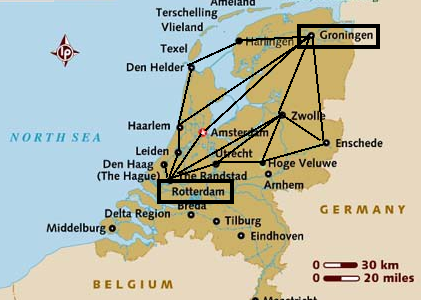
\includegraphics[scale=0.55]{IMAGENES/rotterdam.png}}
\caption{Posibles alternativas para viajar de Rotterdam a Groningen}
\label{fig}
\end{figure}

\subsection{Descripción del algoritmo}

La idea subyacente  [http://ramonlopez.hol.es
/Algoritmo20de20Dijkstra.pdf] consiste en ir explorando \textbf{todos} los caminos más cortos que parten del vértice origen y que llevan a todos los demás vértices. El algoritmo finaliza cuando se alcanza el camino mínimo del nodo origen al resto de nodos.

\begin{figure}[H]
\centerline{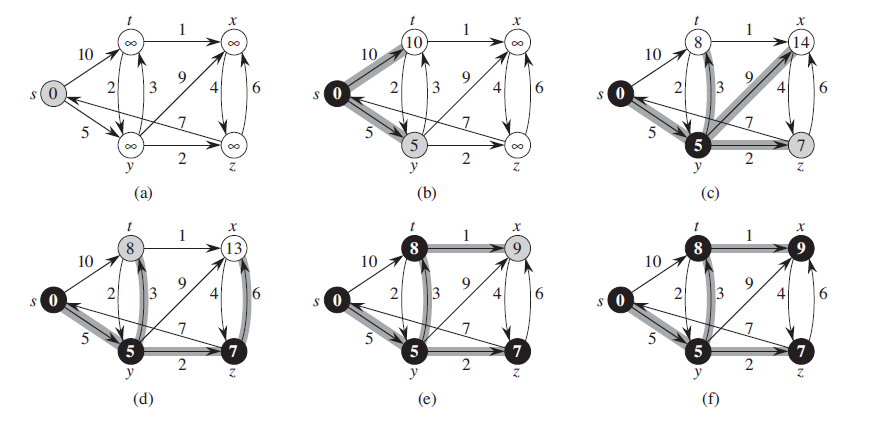
\includegraphics[scale=0.325]{IMAGENES/dijkstra.png}}
\caption{Exploración llevada a cabo por Dijkstra [ref Jatin thaku http://www.codebytes.in/2014/08/dijkstras-algorithm-implementation-in.html]}
\label{fig}
\end{figure}

\begin{center}
\textit{Pseudocódigo}
\end{center}

\begin{enumerate}
\item DIJKSTRA (origen,destino)
\item \hspace{0.5cm} Mientras existan vértices que recorrer:
\item \hspace{1cm} actual = nodoConMínimoCoste()
\item \hspace{1cm} Generamos los hijos, para cada hijo:
\item \hspace{1.15cm} Si no se había generado previamente:
\item \hspace{1.25cm} Lo añadimos al conjunto y actualizamos coste (coste(actual) + coste(actual,hijo))
\item \hspace{1.15cm} Si sí se había generado y el nuevo coste es menor que el que tenía:
\item \hspace{1.25cm} Actualizamos padre y coste
\item \hspace{1cm} Volvemos a 2
\end{enumerate}


\subsection{Propiedades}

Las propiedades del algoritmo de Dijkstra son:
\begin{itemize}

\item Completo. Al recorrer todos los nodos, podemos afirmar que el algoritmo encuentra solución siempre que exista.
\item Óptimo. El algoritmo de Dijkstra encuentra el camino mínimo dados dos nodos. Esta fue la principal propiedad que se trató de satisfacer, la razón de ser de Dijkstra.

\end{itemize}

\subsection{Complejidad}

Para determinar la complejidad computacional [wikipedia] se pueden contar las operaciones realizadas:
\begin{itemize}
\item El algoritmo consiste en n-1 iteraciones (recorrido de todos los nodos).
\item En cada iteración, se identifica el nodo con menor coste y se realiza una suma y comparación para actualizar el coste de los vértices que no se hayan expandido. 2*(n-1) iteraciones
\end{itemize}

Se realizan por tanto un total de $2*(n-1)*(n-1)$. Luego la complejidad del algoritmo es de orden O($n^2$). No obstante, dependiendo de la estructura de datos escogida para almacenar los nodos, las operaciones se podrían realizar más/menos rápidas y por tanto el tiempo empleado variará ligeramente.

Debido a que para cada nodo, almacenamos los caminos más cercanos al resto de los $N$ nodos, la complejidad en espacio es del orden O($N*N$) = O($N^2$) 

\subsection{Experimentación}

Escogiendo aleatoriamente los mapas donde mostrar los resultados obtenemos:
\begin{itemize}
\item Para el mapa \textit{mapa5.csv} partiendo de \textit{(4,16)-celda roja} y queriendo alcanzar \textit{(4,10)-celda amarilla}:

\begin{figure}[H]
 \centering
  \subfloat[En fase de exploración]{
   \label{f:gato}
    \hspace{-0.5mm}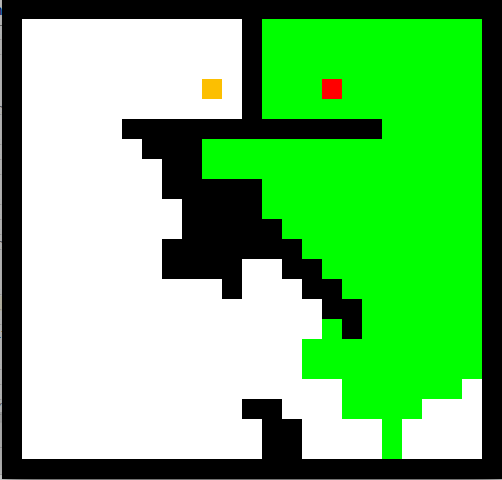
\includegraphics[width=0.225\textwidth]{IMAGENES/dijkstra1.png}}
  \subfloat[Mapa explorado-camino encontrado]{
   \label{f:tigre}
    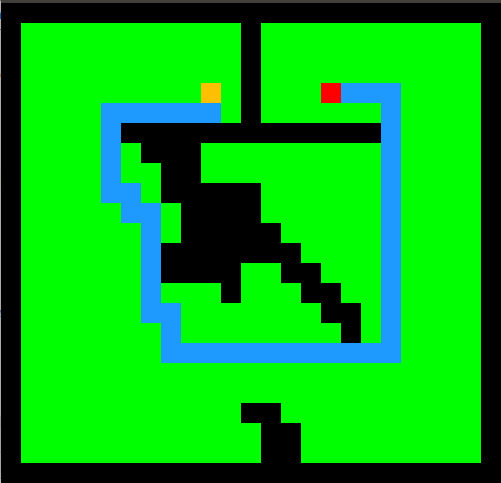
\includegraphics[width=0.225\textwidth]{IMAGENES/dijkstra2.png}}
 \caption{Simulación de Dijkstra en $mapa5.csv$}
 \label{f:animales}
\end{figure}

\item Para el mapa \textit{mapa8.csv} partiendo de \textit{(3,3)-celda roja} y queriendo alcanzar \textit{(11,18)-celda amarilla}:

\begin{figure}[H]
 \centering
  \subfloat[En fase de exploración]{
   \label{f:gato}
    \hspace{-0.5mm}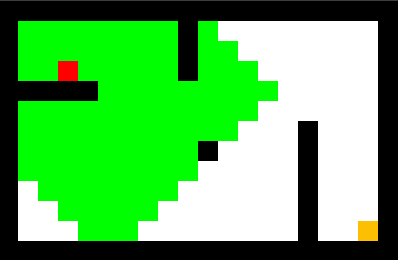
\includegraphics[width=0.235\textwidth]{IMAGENES/dijkstra21.png}}
  \subfloat[Mapa explorado-camino encontrado]{
   \label{f:tigre}
    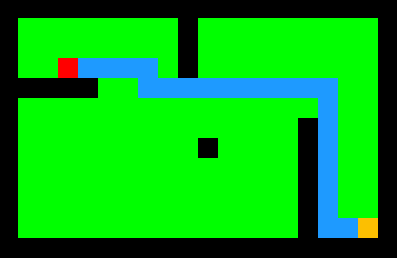
\includegraphics[width=0.235\textwidth]{IMAGENES/dijkstra22.png}}
 \caption{Simulación de Dijkstra en $mapa8.csv$}
 \label{f:animales}
\end{figure}

\end{itemize}

\section{Greedy First Search (GFS)}

\vspace{0.2mm}

\subsection{Descripción del algoritmo}

Estamos ante el método más general de los catalogados algoritmos de búsqueda informados. GFS trata de explorar el grafo expandiendo (en primer lugar) aquellos nodos más prometedores, es decir, que se estima que están más próximos del objetivo.\\


\begin{center}\textit{¿Cómo sabemos cuál es el nodo más prometedor?}\end{center}

\vspace{0.1mm}

El nodo más prometedor será aquel cuya función de evaluación (coste) sea la mínima. En todos los métodos basados en esta técnica, la función de evaluación \textbf{f(n)} incluye una componente heurística, denotada \textbf{h(n)}: 
 \begin{center}
 \textbf{h(n)} = Coste estimado de la distancia entre el nodo n y el nodo objetivo.
 \end{center}

En concreto, GFS utiliza la función de evaluación \[f(n) = h(n)\]

\begin{center}\textit{Pseudocódigo}\end{center}

\begin{enumerate}
\item GFS (q,origen,destino)
\item Mientras que la cola q no esté vacía:
\item \hspace{1cm} actual = nodoConMínimaFunciónEvaluación(q)
\item \hspace{1cm} Si actual = destino: FIN
\item \hspace{1cm} Si No:
\item \hspace{1.25cm} generamos los hijos del nodo actual
\item \hspace{1.25cm} Volvemos a 2
\end{enumerate}

Como vemos, la metodología en la realización de la búsqueda es parecida a la búsqueda en anchura (sección II). Las dos únicas diferencias residen:
\begin{itemize}

\item Línea 3. Mientras que BFS escoge el primer nodo que encuentre en la lista para expandir, GFS escoge el, a priori, más prometedor (menor f(n)).
\item En búsqueda en anchura si no podemos seguir avanzando por un nodo (hijos explorados), retrocedemos. En la versión original de GFS esto no es posible, es decir, no hay backtracking o `vuelta atrás'

\end{itemize}

\subsection{Propiedades}

Para argumentar las propiedades de este algoritmo de búsqueda, se va a utilizar como ejemplo la determinación de caminos entre ciudades del siguiente mapa de Rumanía:

\begin{figure}[H]
\centerline{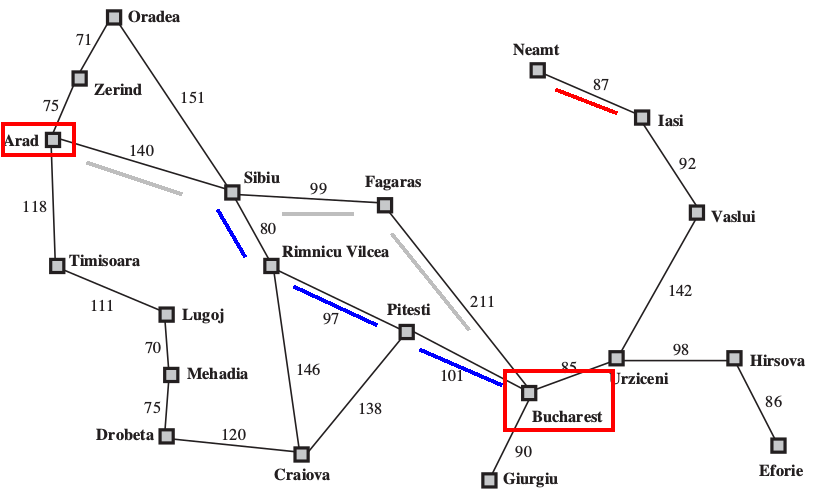
\includegraphics[scale=0.3]{IMAGENES/RUMANIA.png}}
\caption{Mapa de ciudades de Rumanía}
\label{fig}
\end{figure}

Supongamos que queremos que nuestro robot vaya desde Arad a Bucharest. Para que GFS funcione, necesitamos conocer para cada ciudad $C_{i}$, \textbf{h($c_{i}$)}. Esta información se recoge en la tabla:

\begin{figure}[H]
\centerline{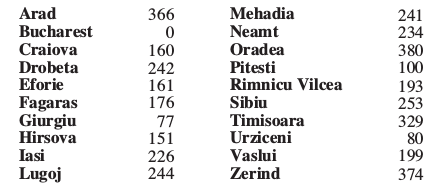
\includegraphics[scale=0.4]{IMAGENES/tablagfs.png}}
\caption{Heurísticas para GFS [ref libro]}
\label{fig}
\end{figure}

Para trazar el camino más corto entre Arad-Bucharest, GFS expandirá Sibiu-Fagaras-Bucharest (camino gris) que como podemos apreciar, no es el óptimo. El camino óptimo sería Arad-Sibiu-Rimnicu Vilcea-Pitesti-Bucharest (camino azul).
\begin{figure}[H]
\centerline{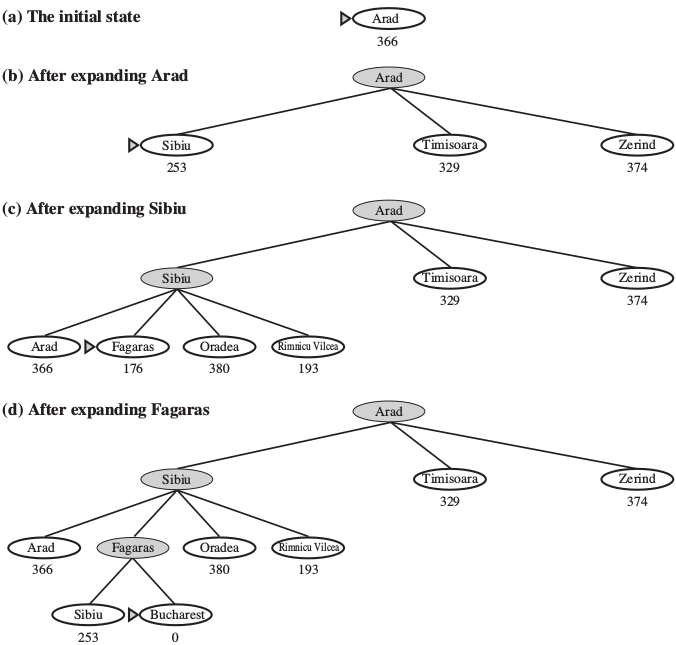
\includegraphics[scale=0.35]{IMAGENES/gfs.png}}
\caption{Exploración de GFS [ref libro]}
\label{fig}
\end{figure}

Además si intentáramos trazar un camino Iasi-Fagaras, el algoritmo se quedaría estancado en Neamt.\\

Por tanto, podemos concluir:
\begin{itemize}
\item GFS no es óptimo, es decir, no asegura encontrar el camino mínimo entre dos puntos.
\item GFS no es completo, es decir, puede no encontrar camino alguno entre dos nodos.
\end{itemize}


\subsection{Complejidad}

Las dos propiedades negativas previamente descritas nos hacen preguntarnos si realmente es útil el uso de GFS. Es aquí donde podemos argumentar:
\begin{enumerate}
\item Debido a que no realiza backtracking, la complejidad en espacio requerida por el algoritmo se reduce notablemente.
\item Se reduce además la complejidad en tiempo sustancialmente si se hace uso de una buena función heurística.
\end{enumerate}

\subsection{Experimentación}

En la fase de experimentación se desarrollaron dos versiones de GFS:
\begin{enumerate}
\item gfs\_incomplete . Versión original de GFS que tal y como hemos explicado puede no encontrar el camino.
\item gfs\_complete . Versión completa de GFS.
\end{enumerate}

El resultado obtenido para el mapa \textit{mapa7.csv} partiendo de (4,3)-celda roja y queriendo alcanzar (20,20)-celda amarilla con \textit{gfs\_incomplete} es:

\begin{figure}[H]
\centering
\includegraphics[scale=0.4]{IMAGENES/gfsESTANCADO2.png}
\caption{Exploración \textit{gfs\_incomplete}}
\label{fig}
\end{figure}

Como vemos, el algoritmo no ha sido capaz de encontrar el camino (sea o no mínimo). Es por ello que se probó con la segunda versión implementada obteniendo:

\begin{figure}[H]
 \centering
  \subfloat[Exploración]{
   \label{f:gato}
    \hspace{-0.5mm}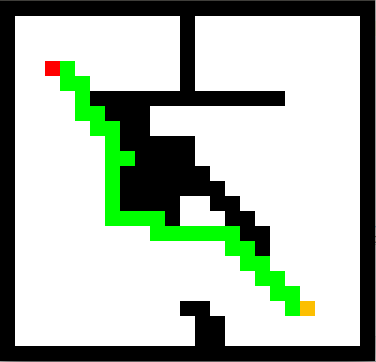
\includegraphics[width=0.225\textwidth]{IMAGENES/gfsC1.png}}
  \subfloat[Camino encontrado]{
   \label{f:tigre}
    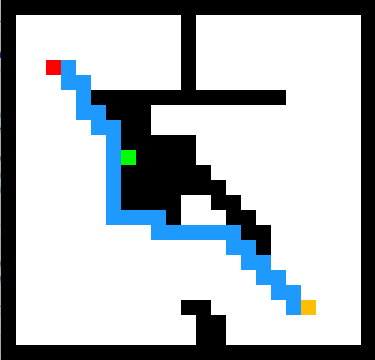
\includegraphics[width=0.225\textwidth]{IMAGENES/gfsC2.png}}
 \caption{Exploración y camino encontrado por \textit{gfs\_complete}}
 \label{f:animales}
\end{figure}

El resultado de \textit{gfs\_complete} para el \textit{mapa5.csv} y los puntos: (4,16) Origen - (4,10) Destino:
\begin{figure}[H]
 \centering
  \subfloat[Exploración]{
   \label{f:gato}
    
\includegraphics[width=0.225\textwidth]{IMAGENES/gfsC11.png}}
  \subfloat[Camino encontrado]{
   \label{f:tigre}
    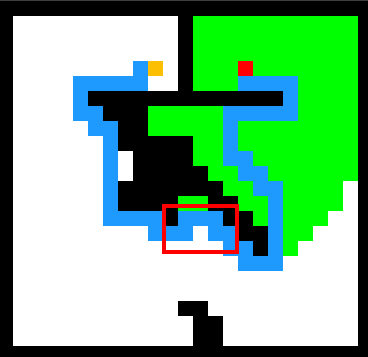
\includegraphics[width=0.225\textwidth]{IMAGENES/gfsC12.png}}
 \caption{Exploración y camino encontrado por \textit{gfs\_complete}}
 \label{f:animales}
\end{figure}

Como vemos, \textit{gfs\_complete} encuentra el camino, pero sigue sin encontrar el óptimo. La zona rectangular roja en la figura 5.(b) lo pone de manifiesto. Una variante de algoritmos greedy que sí que consigue encontrar el camino óptimo es A*.

\section{A*}

\subsection{Descripción del algoritmo}

A* es un algoritmo muy popular usado en planificación de caminos. Fue publicado por primera vez en 1968 [wikipedia] por los autores \textit{Peter Hart},\textit{Nils Nilsson} y \textit{Bertram Raphael}.\\

El secreto del éxito de A* [ref http://theory.stanford.edu/~amitp
/GameProgramming/AStarComparison.html] es que combina:
\begin{itemize}
\item La información que usa Dijkstra (favorecer a los nodos más cercanos al origen)
\item La información heurística que GFS usa (favorecer a los nodos más cercanos al destino)
\end{itemize}

Gracias a ello, A* podría usarse para encontrar caminos óptimos (tal y como hace Dijkstra) usando heurísticas (tal y como GFS hace) y por tanto, en el caso más simple, es tán rápido como GFS.\\

En definitiva, A* examina cada nodo con la función de evaluación: $f(n) = g(n) + h(n)$ , donde:
\begin{itemize}
\item $g(n)$ Es el coste exacto desde origen hasta el nodo $n$.
\item $h(n)$ Es una estimación heurística del coste del camino desde $n$ hasta el destino.
\end{itemize}
\begin{center}
\textit{Pseudocódigo}
\end{center}
\begin{enumerate}
\item A* (origen,destino)
\item \hspace{0.05cm} Definimos CERRADOS = nodos evaluados
\item \hspace{0.05cm} Definimos ABIERTOS = nodos no evaluados
\item \hspace{0.05cm} Añadir(ABIERTOS,origen)
\item \hspace{0.05cm} Mientras que ABIERTOS no esté vacía:
\item \hspace{0.1cm} nodoM = Nodo con menor f(n) = g(n) + h(n)
\item \hspace{0.1cm} Si nodoM = destino : FIN
\item \hspace{0.15cm} Eliminamos nodoM de ABIERTOS
\item \hspace{0.15cm} Añadimos nodoM a CERRADOS
\item \hspace{0.15cm} Generamos los hijos del nodoM
\item \hspace{0.15cm} Para cada hijo:
\item \hspace{0.2cm} Si el hijo está en CERRADOS : Volvemos a 5
\item \hspace{0.25cm} d = Distancia de origen al hijo
\item \hspace{0.25cm} Si hijo no está en ABIERTOS:
\item \hspace{0.35cm} Añadir(ABIERTOS,hijo)
\item \hspace{0.25cm} Si d $<$ Coste Anterior que tenía guardado hijo:
\item \hspace{0.3cm} Actualizamos el hijo : Ponemos su mejor padre nodoN
\item \hspace{0.3cm} Actualizamos f(n) del hijo y volvemos a 5
\end{enumerate}

\begin{figure}[H]
\centerline{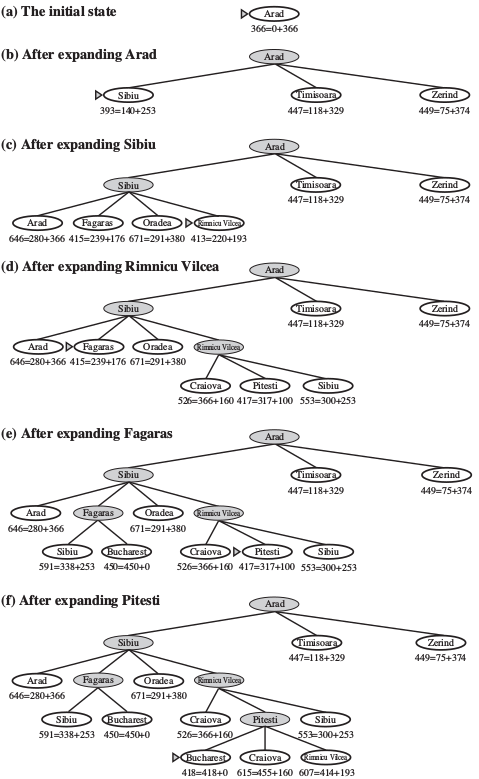
\includegraphics[scale=0.4505]{IMAGENES/A*.png}}
\caption{Exploración de A* [ref libro]}
\label{fig}
\end{figure}

Vemos como en la figura anterior (Fig.11) cada nodo se etiqueta con f(n) = g(n) + h(n).


\subsection{Propiedades}
Las propiedades [wikipedia][https://cs.stanford.edu/people
/eroberts/courses/soco/projects/2003-04/intelligent-search/astar.html] de A* son:
\begin{itemize}
\item El algoritmo es completo. Gracias a ir almacenando los sucesores del mejor nodo en ABIERTOS, si el camino no puede seguir por un nodo, realiza un backtracking al siguiente nodo con mejor f(n).
\item El algoritmo garantiza encontrar la solución óptima sii la heurística de la que hace uso es \textit{admisible} (Una heurística \textit{h} es admisible si la estimación h(n) nunca sobreestima la distancia real del nodo n al nodo destino).\\
\begin{center}$\forall n  \hspace{0.1cm} h(n) <= CosteReal(n,destino)$\end{center}
\end{itemize}

\subsection{Complejidad}

En lo que respecta a la complejidad [wikipedia] de A*:
\begin{itemize}
\item La complejidad \textit{computacional} está íntimamente relacionada con la calidad de la heurística que se utilice.
\begin{itemize}
\item En el peor de los casos exponencial : O($b^d$).
\item En el mejor de los casos polinomial.
\end{itemize}

\item La complejidad en \textit{memoria} es su mayor problema ya que es exponencial respecto al tamaño del problema.
\end{itemize}

\subsection{Experimentación}

Escogiendo aleatoriamente los mapas donde mostrar los resultados obtenemos:
\begin{itemize}
\item Para el mapa \textit{mapa6.csv} partiendo de \textit{(3,3)-celda roja} y queriendo alcanzar \textit{(11,18)-celda amarilla}:

\begin{figure}[H]
 \centering
  \subfloat[En fase de exploración]{
   \label{f:gato}
    \hspace{-0.5mm}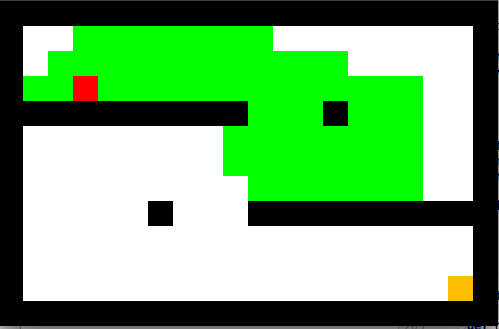
\includegraphics[width=0.225\textwidth]{IMAGENES/astar1.png}}
  \subfloat[Mapa explorado-camino encontrado]{
   \label{f:tigre}
    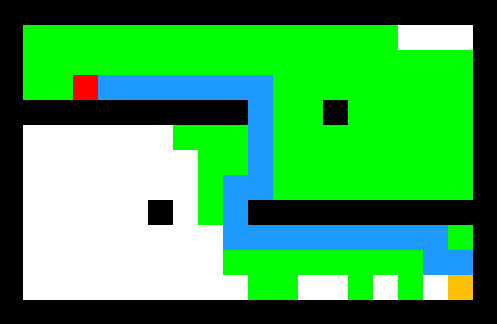
\includegraphics[width=0.225\textwidth]{IMAGENES/astar2.png}}
 \caption{Simulación de A* en $mapa6.csv$}
 \label{f:animales}
\end{figure}

\item Para el mapa \textit{mapa5.csv} partiendo de \textit{(4,16)-celda roja} y queriendo alcanzar \textit{(4,10)-celda amarilla}:

\begin{figure}[H]
 \centering
  \subfloat[En fase de exploración]{
   \label{f:gato}
    \hspace{-0.5mm}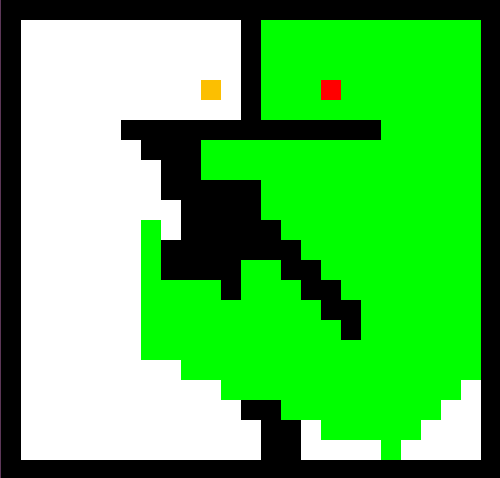
\includegraphics[width=0.235\textwidth]{IMAGENES/astar21.png}}
  \subfloat[Mapa explorado-camino encontrado]{
   \label{f:tigre}
    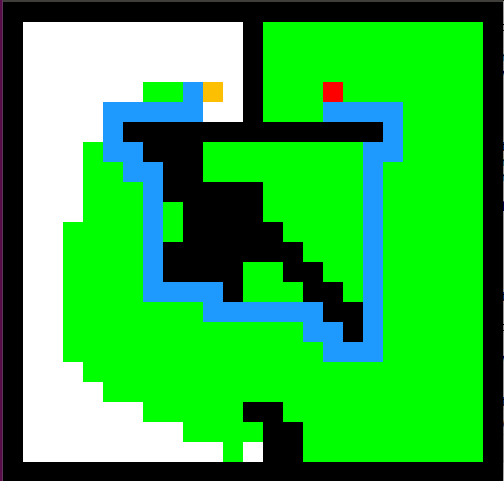
\includegraphics[width=0.235\textwidth]{IMAGENES/astar22.png}}
 \caption{Simulación de A* en $mapa5.csv$}
 \label{f:animales}
\end{figure}

\end{itemize}


\section{Rapidly exploring random tree (rrt)}

En esta sección se presenta un enfoque de algoritmos de planificación basado en muestreo.\\
 
La idea fudamental de este tipo de planificadores es la de aproximar la conectividad del espacio de configuraciones mediante una estructura de grafos. El espacio a explorar es muestreado, generando estados que formarán los vertices de dicho grafo. Las líneas que unen los vértices del grafo denontan segmentos de camino válidos.\\
 
El objetivo es capturar la conectividad del espacio de configuración del agente o robot en movimiento a través de un muestreo aleatorio. 
Los árboles de exploración aleatoria rápida (Rapidly Exploring Random Tree o RRT) fueron desarrollados por Steven M.LaValle y James J.Kuffner Jr. Pueden ser vistos como una técnica para generar trayectorias de bucle abierto con el fin de buscar, de manera eficiente, los espacios de alta dimensión no convexos mediante la construcción aleatoria de un árbol de relleno de espacio.  

\subsection{Descripción del algoritmo}

La idea de un RRT es hacer crecer un arbol de búsqueda, que mejore gradualmente, arraigado en la configuración inicial utilizando muestras aleatorias del espacio de búsqueda. A medida que se toma cada muestra, se intenta realizar una conexión entre ella y el estado más cercano en el árbol. Si la conexión es factible (pasa completamente a través del espacio libre y obedece cualquier restricción), se produce la adición del nuevo estado al árbol. \\

La longitud de la conexión entre el árbol y un nuevo estado está frecuentemente limitada por un factor de crecimiento. Si la muestra aleatoria se encuentra a una distancia mayor de su estado más cercano en el árbol de lo que permite este límite, se genera un nuevo estado a la distancia máxima del árbol a lo largo de la línea hasta la muestra aleatoria en lugar de la muestra aleatoria en sí. Las muestras aleatorias se pueden ver como control de la dirección del crecimiento del árbol, mientras que el factor de crecimiento determina su tasa. Esto mantiene el sesgo de relleno de espacio del RRT al tiempo que limita el tamaño del crecimiento incremental.\\

El crecimiento de RRT puede estar sesgado al aumentar la probabilidad de muestrear estados de un área específica. La mayoría de las implementaciones prácticas de las RRT hacen uso de esto para guiar la búsqueda hacia los objetivos de planificación de problemas. Esto se logra introduciendo una pequeña probabilidad de muestrear la meta al procedimiento de muestreo estatal. Cuanto mayor es esta probabilidad, más veloz crece el árbol hacia la meta.\\

El empleo de este tipo de algoritmos en planificadores, presenta varias etapas, las cuáles se encuentran representadas en la Fig 14.

\begin{figure}[H]
\centerline{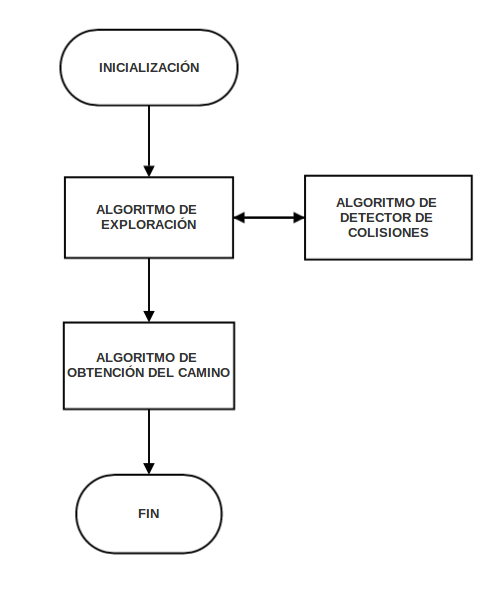
\includegraphics[scale=0.4]{IMAGENES/flujo.png}}
\caption{Etapas de RRT [ref libro]}
\label{fig}
\end{figure}

En el estado de inicialización se realizan las configuraciones necesarias del algoritmo, tales como la lectura del espacio de estados, la determinación de punto origen del robot, del destino etc.

\begin{center}
\textit{ALGORITMO DE EXPLORACIÓN}
\end{center}

El segundo estado que presenta el diagrama de flujo, trata el algoritmo de exploración utilizando un árbol aleatorio de búsqueda.\\

El pseudocódigo que permite la construcción de un árbol de exploración básico en un espacio de configuraciones sin obstáculos (donde todo el espacio es completamente libre).

\begin{enumerate}
\item SIMPLE\_RDT (q0)
\item \hspace{0.05cm} Iniciamos el grafo G con q0.
\item \hspace{0.05cm} Desde i=1 hasta NumeroIteraciones:
\item \hspace{0.1cm} Añadimos a G un nuevo vértice aleatorio generado : $\alpha (i)$
\item \hspace{0.1cm} $q_n \Leftarrow MasCercano(S(G),\alpha (i))$
\item \hspace{0.1cm} Añadir línea que une $q_n \- \alpha (i)$

\end{enumerate}

En resumidas cuentas, el algoritmo requiere la disponibilidad de una secuencia densa, $\alpha$, y se conecta iterativamente desde $\alpha (i)$ al punto más cercano entre todos los alcanzados por el arbol, G.\\

En la Fig.15 se muestra en (a) un arbol que ha sido construido estableciendo un punto inicial q0. En (b) un nuevo eje aleatoriamente es añadido conectándose desde $\alpha (i)$ al punto más cercano en S, vértice $q_n$.

\begin{figure}[H]
\centerline{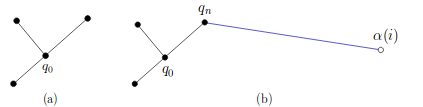
\includegraphics[scale=0.6]{IMAGENES/RRT1.png}}
\caption{Crecimiento del árbol (1)}
\label{fig}
\end{figure}

\begin{figure}[H]
\centerline{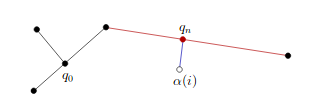
\includegraphics[scale=0.7]{IMAGENES/RRT2.png}}
\caption{Crecimiento del árbol (2)}
\label{fig}
\end{figure}

En la Fig.17 se muestra la visualización en un espacio libre de obstáculos de la misma simulación una vez transcurridas 3500 y 6500 iteraciones.

\begin{figure}[H]
 \centering
  \subfloat[Tras 3500 iteraciones]{
   \label{f:gato}
    \hspace{-0.5mm}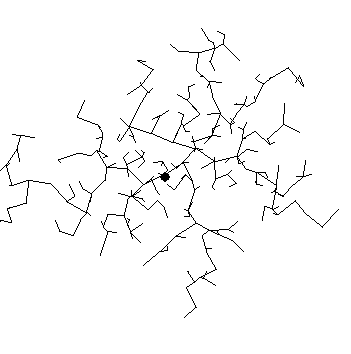
\includegraphics[width=0.25\textwidth]{IMAGENES/RRT3.png}}
  \subfloat[Tras 6500 iteraciones]{
   \label{f:tigre}
    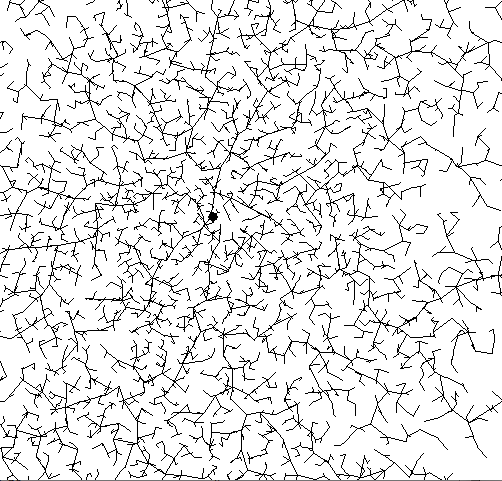
\includegraphics[width=0.25\textwidth]{IMAGENES/RRT4.png}}
 \caption{Simulación en mapa libre de obstáculos}
 \label{f:animales}
\end{figure}

Una vez se ha muestreado todo el espacio libre del espacio de configuraciones, se obtiene el camino mediante  la obtención de los padres de cada nodo.

\subsection{Propiedades}

Las propiedades del RRT son:
\begin{itemize}
\item Probabilísticamente completos. A medida que crece el número de iteraciones, la probabilidad de encontrar una ruta de solución tiende a la unidad si al menos existe una solución, de lo contrario el algortimo se repite para siempre.
\item Algoritmo no óptimo. Debido a la naturaleza aleatoria de los árboles de búsqueda, este tipo de planificadores no obtienen la ruta más óptima ya que en cada simulación, los nodos serán diferentes y por tanto el camino también lo será.
\end{itemize}

\subsection{Complejidad}

Para determinar la complejidad del tiempo (time complexity) será de O(M(N+K), donde M es el número de iteraciones, N, el tiempo empleado en encontrar el nodo más cercado, qn , y K el tiempo empleado en conectar ambos nodos.

\subsection{Experimentación}
Escogiendo aleatoriamente los mapas donde mostrar los resultados, obtenemos:
\begin{itemize}

\item Para el mapa \textit{mapa3.csv} partiendo de \textit{(5,11)-celda roja} y queriendo alcanzar \textit{(5,15)-celda amarilla}:

\begin{figure}[H]
  \subfloat[En fase de exploración]{
   \label{f:gato}
    \hspace{-0.5mm}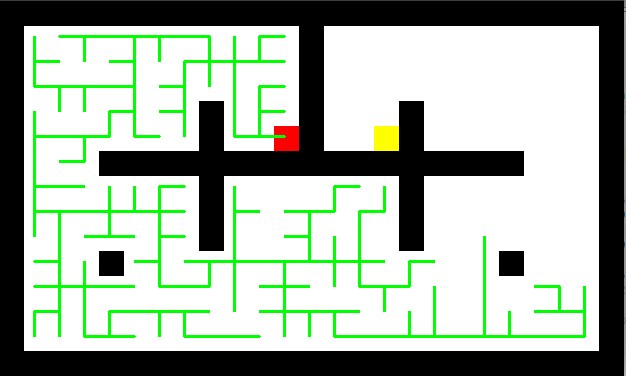
\includegraphics[width=0.245\textwidth]{IMAGENES/rrtE1.png}}
  \subfloat[Mapa explorado-camino encontrado]{
   \label{f:tigre}
    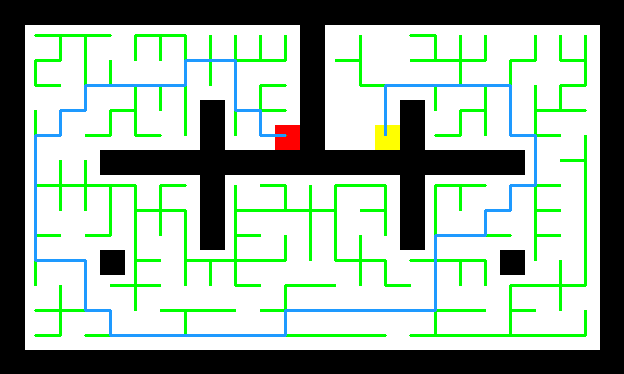
\includegraphics[width=0.245\textwidth]{IMAGENES/rrtE12.png}}
 \caption{Simulación de RRT en $mapa5.csv$}
 \label{f:animales}
\end{figure}

\item Para el mapa \textit{mapa8.csv} partiendo de \textit{(3,3)-celda roja} y queriendo alcanzar \textit{(11,18)-celda amarilla}:

\begin{figure}[H]
  \subfloat[En fase de exploración]{
   \label{f:gato}
    \hspace{-0.5mm}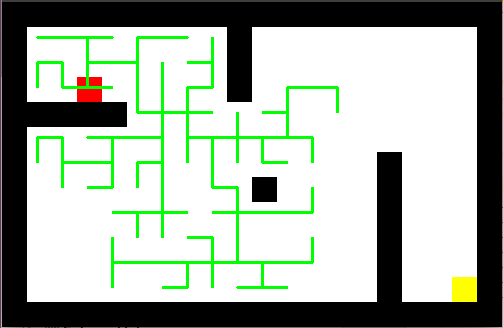
\includegraphics[width=0.245\textwidth]{IMAGENES/rrtE21.png}}
  \subfloat[Mapa explorado-camino encontrado]{
   \label{f:tigre}
    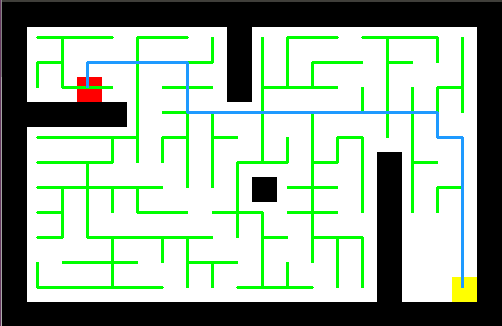
\includegraphics[width=0.245\textwidth]{IMAGENES/rrtE22.png}}
 \caption{Simulación de RRT en $mapa8.csv$}
 \label{f:animales}
\end{figure}

\end{itemize}

\section*{References}

Please number citations consecutively within brackets \cite{b1}. The 
sentence punctuation follows the bracket \cite{b2}. Refer simply to the reference 
number, as in \cite{b3}---do not use ``Ref. \cite{b3}'' or ``reference \cite{b3}'' except at 
the beginning of a sentence: ``Reference \cite{b3} was the first $\ldots$''

Number footnotes separately in superscripts. Place the actual footnote at 
the bottom of the column in which it was cited. Do not put footnotes in the 
abstract or reference list. Use letters for table footnotes.

Unless there are six authors or more give all authors' names; do not use 
``et al.''. Papers that have not been published, even if they have been 
submitted for publication, should be cited as ``unpublished'' \cite{b4}. Papers 
that have been accepted for publication should be cited as ``in press'' \cite{b5}. 
Capitalize only the first word in a paper title, except for proper nouns and 
element symbols.

For papers published in translation journals, please give the English 
citation first, followed by the original foreign-language citation \cite{b6}.

\begin{thebibliography}{00}
\bibitem{b1} G. Eason, B. Noble, and I. N. Sneddon, ``On certain integrals of Lipschitz-Hankel type involving products of Bessel functions,'' Phil. Trans. Roy. Soc. London, vol. A247, pp. 529--551, April 1955.
\bibitem{b2} J. Clerk Maxwell, A Treatise on Electricity and Magnetism, 3rd ed., vol. 2. Oxford: Clarendon, 1892, pp.68--73.
\bibitem{b3} I. S. Jacobs and C. P. Bean, ``Fine particles, thin films and exchange anisotropy,'' in Magnetism, vol. III, G. T. Rado and H. Suhl, Eds. New York: Academic, 1963, pp. 271--350.
\bibitem{b4} K. Elissa, ``Title of paper if known,'' unpublished.
\bibitem{b5} R. Nicole, ``Title of paper with only first word capitalized,'' J. Name Stand. Abbrev., in press.
\bibitem{b6} Y. Yorozu, M. Hirano, K. Oka, and Y. Tagawa, ``Electron spectroscopy studies on magneto-optical media and plastic substrate interface,'' IEEE Transl. J. Magn. Japan, vol. 2, pp. 740--741, August 1987 [Digests 9th Annual Conf. Magnetics Japan, p. 301, 1982].
\bibitem{b7} M. Young, The Technical Writer's Handbook. Mill Valley, CA: University Science, 1989.
\end{thebibliography}
\vspace{12pt}
\color{red}


\end{document}
